\documentclass[english,hebrew]{article}
\usepackage[HE8,T1]{fontenc}
\usepackage[utf8]{inputenc}
\setcounter{secnumdepth}{-2}
\setlength{\parindent}{0bp}
\usepackage{calc}
\usepackage{amsmath}
\usepackage{amsthm}
\usepackage{amssymb}
\usepackage{graphicx}

\makeatletter
\@ifundefined{date}{}{\date{}}
\usepackage{graphicx}
\usepackage{geometry}
\newcommand{\limi}{\underset{n\rightarrow\infty}{\lim}}
\newcommand{\limxz}{\underset{x\rightarrow x_{0}}{\lim}}
\newcommand{\limfxz}{\underset{x\rightarrow x_{0}}{\lim}f(x)}
\newcommand{\limfxm}{\underset{x\rightarrow x_{0}^{-}}{\lim}f(x)}
\newcommand{\limfxp}{\underset{x\rightarrow x_{0}^{+}}{\lim}f(x)}
\newcommand{\limxm}{\underset{x\rightarrow x_{0}^{-}}{\lim}}
\newcommand{\limxp}{\underset{x\rightarrow x_{0}^{+}}{\lim}}
\newcommand{\sqrm}{M_{m\times m}(\mathbb{F})}
\newcommand{\seqa}{(a_{n})_{n=1}^{\infty}}
\newcommand{\seqx}{(x_{n})_{n=1}^{\infty}}
\newcommand{\funcdr}{f:D\rightarrow\mathbb{R}}
\newcommand{\der}{\limxz\frac{f(x)-f(x_{0})}{x-x_{0}}}
\usepackage[all]{pdfprivacy}

\makeatother

\usepackage{babel}
\begin{document}
\newgeometry{top=1cm, bottom=2cm, left=1cm, right=1cm}
\title{אלגברה ליניארית {\beginL 2\endL} - הרצאה {\beginL 1\endL}}
\author{נעם לב}
\date{\L{$11.10.2026$}}

\maketitle
\noindent\fbox{\begin{minipage}[t]{1\columnwidth - 2\fboxsep - 2\fboxrule}%
\begin{center}
האוניברסיטה העברית \textbar{} אלגברה ליניארית ){\beginL 2\endL}( -
\L{$80135$} \textbar{} סמסטר{\small{} }{\beginL 2027\endL}{\small{} }א'
)תשפ\textquotedblleft ז א'( \textbar{} מרצה: פרופסור יבגני סטרחוב
\par\end{center}%
\end{minipage}}
\begin{center}
הסיכום הוא לא רשמי ולא עבר אישור של הסגל, על כן אין להשתמש בו )ובין
השאר במספור שלו ובשמות הטענות שבו( כמקור רשמי. אם ישנן טעויות, הן
שלי ולא של הסגל.
\par\end{center}

\medskip{}

\tableofcontents{}

\newpage{}

\part{מנהלה}

ספרות מומלצת עבור הקורס: \L{$\text{Linear Algebra Done Right by Axler}$},
נמצא בחינם באינטרנט וקיימת גם גרסה מתורגמת לעברית.

שעת קבלה: יום ד', חמש עד שש אחה\textquotedblleft צ. 

נתמקד בהעתקות לינאריות מ-מ\textquotedblleft ו לעצמו, ובעיקר מעל \L{$\mathbb{R}$}
ו-\L{$\mathbb{C}$}.

דברים שחשוב לנרענן מלינארית 1: מטריצה מייצגת של ה\textquotedblleft ל,
ה\textquotedblleft ל הפיכה היא חח\textquotedblleft ע ועל, חישוב ומציאת
בסיס לגרעין ותמונה. 

\part{רענון הגדרות )היה בתרג\textquotedblleft פ(}

\section{הומומורפיזם}

הומומורפיזם הוא ה\textquotedblleft ל מ-מ\textquotedblleft ו ל-מ\textquotedblleft ו
כאשר שניהם מעל אותו שדה \L{$\mathbb{F}$}. קבוצת ההומומורפיזמים היא\L{%
\[
\text{\text{Hom}(V,W)}=\left\{ T\mid T:V\rightarrow W\text{ is a LT}\right\} 
\]
}%

היא כשלעצמה מ\textquotedblleft ו מעל \L{$\mathbb{F}$}.

\section{אנדומורפיזם}

הומומורפיזם ממ\textquotedblleft ו לעצמו. קבוצת האנדומורפיזמים של מ\textquotedblleft ו
\L{$V$} היא\L{%
\[
\text{\text{End}(V)}=\text{\text{Hom}(V,V)}
\]
}%

\section{איזומורפיזם}

ה\textquotedblleft ל \L{$T:V\rightarrow W$} תיקרא איזומורפיזם אם
היא חח\textquotedblleft ע ועל. אם קיימת כזו, אז \L{$W$} ממימד סופי
אם\textquotedblleft ם גם \L{$V$} ממימד סופי, ובמקרה זה המימדים שלהם
שווים\L{%
\[
\dim(V)=\dim(W)
\]
}%

\L{$T$} איזומורפיזם אם\textquotedblleft ם קיימת ה\textquotedblleft ל
\L{$S:W\rightarrow V$} כך ש-\L{%
\[
TS=\text{Id}_{W}
\]
}%
\L{%
\[
ST=\text{Id}_{V}
\]
}%

\section{הקשר בין הומומורפיזם למטריצה}

\L{$\left[\clubsuit\right]$} יהיו \L{$V,W$} מ\textquotedblleft ו
ממימד סופי מעל \L{$\mathbb{F}$}, עם \L{$\dim(V)=n$} ו- \L{$\dim(W)=m$}.

יהיו \L{$\mathcal{B}=\left(u_{1},\dots,u_{n}\right)$} בסיס של \L{$V$}
ו-\L{$\mathcal{C}$} בסיס של \L{$W$}.

אז לכל \L{$T\in\text{\text{Hom}(V,W)}$} קיימת מטריצה \L{%
\[
\left[T\right]_{\mathcal{C}}^{\mathcal{B}}\in M_{m\times n}\left(\mathbb{F}\right)
\]
}%
כך שהעמודה ה-\L{$j$} שלה היא \L{$\left[T\left(u_{j}\right)\right]_{\mathcal{C}}$}
ולכל \L{$v\in V$} מתקיים\L{%
\[
\left[T(v)\right]_{\mathcal{C}}=\left[T\right]_{\mathcal{C}}^{\mathcal{B}}\left[v\right]_{\mathcal{B}}
\]
}%

\L{$\left[\diamondsuit\right]$} נוכל להסתכל על ה\textquotedblleft ל
שלוקחת ה\textquotedblleft ל \L{$T$} ומחזירה את המטריצה המייצגת אותה.

ה\textquotedblleft ל זו היא איזומורפיזם של מ\textquotedblleft ו. 

בנוסף, אם ה\textquotedblleft ל זו מתאימה לה\textquotedblleft ל \L{$T:V\rightarrow W$}
מטריצה עם \L{$m$} שורות ו-\L{$n$} עמודות, אז \L{%
\[
\dim\text{Hom}\left(V,W\right)=mn
\]
}%
\L{$\left[\heartsuit\right]$} עבור \L{$S:W\rightarrow U$} עם בסיס
\L{$\mathcal{D}$} של \L{$U$} מתקיים\L{%
\[
\left[ST\right]_{\mathcal{D}}^{\mathcal{B}}=\left[S\right]_{\mathcal{D}}^{\mathcal{C}}\left[T\right]_{\mathcal{C}}^{\mathcal{B}}
\]
}%

\L{$\left[\spadesuit\right]$} אם \L{$T\in\text{End\ensuremath{\left(V\right)}}$},
החלפת בסיס נותנת מטריצות דומות\L{%
\[
\left[T\right]_{\mathcal{B}'}=P^{-1}\left[T\right]_{\mathcal{B}}P
\]
}%
 כאשר \L{$P=\left[\text{Id}_{V}\right]_{\mathcal{B}}^{\mathcal{B}'}$}
היא מטריצת המעבר מ-\L{$\mathcal{B}'$} ל-\L{$\mathcal{B}$}. 

\L{$\left[\triangle\right]$} \L{$T$} הוא איזומורפיזם אם\textquotedblleft ם
\L{$\left[T\right]_{\mathcal{C}}^{\mathcal{B}}$} הפיכה )ובפרט \L{$m=n$}(.
במקרה זה \L{%
\[
\left[T^{-1}\right]_{\mathcal{B}}^{\mathcal{C}}=\left(\left[T\right]_{\mathcal{C}}^{\mathcal{B}}\right)^{-1}
\]
}%

\part{הגדרה - אופרטור לינארי}

עבור מ\textquotedblleft ו )מרחב וקטורי( \L{$V$} מעל \L{$\mathbb{F}$}
\L{$(\mathbb{F}\underset{(*)}{=}\mathbb{C},\mathbb{R})$}, הקבוצה
הבאה\L{%
\[
\mathcal{L}(V)=\left\{ T:V\rightarrow V:T\text{ is a LT}\right\} =\text{Hom}(V,V)=\text{Hom}_{\mathbb{F}}(V,V)
\]
}%
היא קבוצת האופרטורים הלינאריים במרחב \L{$V$}.

\L{$(*)$} כמו בספר של אקסלר, בד\textquotedblleft כ \L{$\mathbb{F}$}
יתייחס לשדות \L{$\mathbb{C}$} ו-\L{$\mathbb{R}$}.

\section{\L{$\text{Null, Range}$}}

יהי \L{$V$} מ\textquotedblleft ו מעל \L{$\mathbb{F}$} ותהא \L{$T\in\mathcal{L}(V)$}.
אז

\L{%
\[
\text{Null}(T)\overset{\text{def}}{=}\left\{ v\in V:T(v)=0_{V}\right\} 
\]
}%
\L{%
\[
\text{Range}(T)\overset{\text{def}}{=}\left\{ v\in V:\exists v'\in V\text{ s.t. }T(v')=v\right\} 
\]
}%

)אלה הגרעין והתמונה מלינארית {\beginL 1\endL}, \L{$\text{Null}$}
זה קרנל(.

\part{הגדרה - \L{$\text{Invariant subspace of \ensuremath{T}}$} - תת-מרחב
שמור תחת \L{$T$}}

עבור מ\textquotedblleft ו \L{$V$} מעל שדה \L{$\mathbb{F}$}, תמ\textquotedblleft ו
\L{$U$} של \L{$V$}, ו- \L{$T\in\mathcal{L}(V)$}, אם \L{%
\[
\forall u\in U:T(u)\in U
\]
}%
 אז נאמר כי \L{$U$} הוא תמ\textquotedblleft ו שמור תחת \L{$T$}.

במילים אחרות, \L{$T(U)\subseteq U$} . 

\section{דוגמאות}

\subsection{דוגמה{\normalsize{} }{\beginL 1\endL}}

יהי \L{$T\in\mathcal{L}(V)$}. אז \L{$V$} ו-\L{$\{0_{V}\}$} שניהם
תמ\textquotedblleft ו שמורים תחת \L{$T$}.

\subsubsection{הוכחה}

מעצם הגדרת אופרטור לינארי, \L{$T(V)\subseteq V$} וגם \L{$T\left(0_{V}\right)=0_{V}$}.

\subsection{דוגמה{\normalsize{} }{\normalsize{\beginL 2}\endL}}

\L{$V=\mathbb{R}^{3}$}, \L{$T_{\theta}$} - סיבוב בזווית \L{$\theta\notin\left\{ k\pi:k\in\mathbb{Z}\right\} $}
סביב ציר \L{$\hat{z}$} נגד כיוון השעון.

\L{$T_{\theta}\in\mathcal{L}(\mathbb{R}^{3})$}. 
\begin{center}
\L{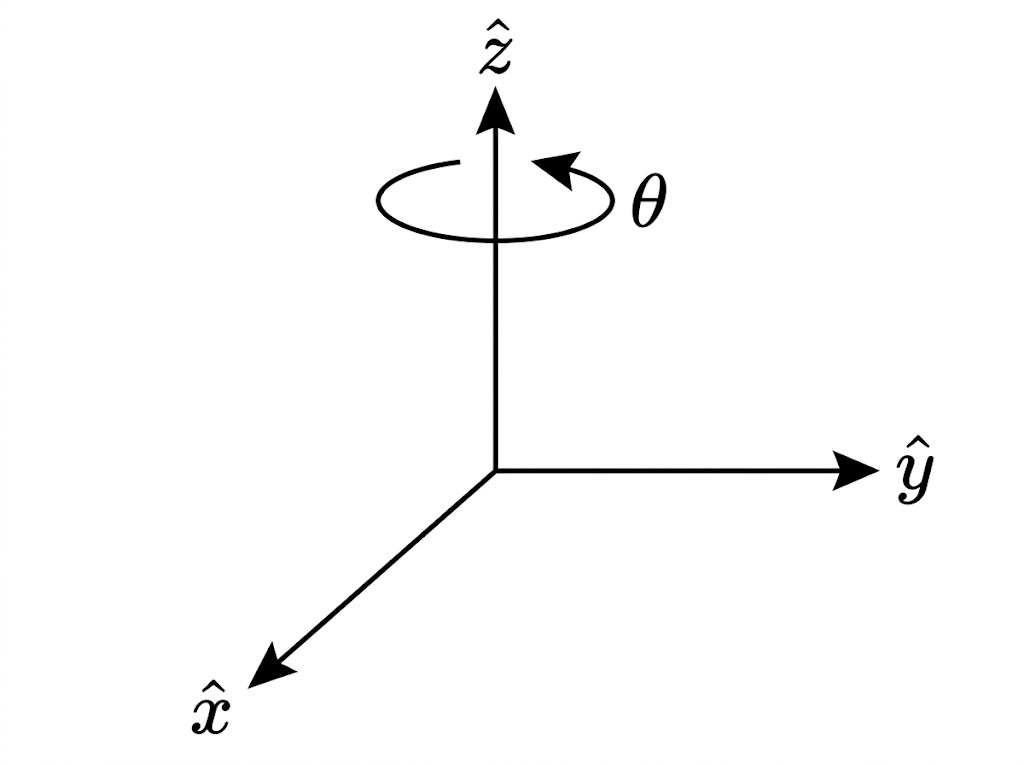
\includegraphics[scale=0.25]{pasted1}}
\par\end{center}

אז\L{%
\[
U_{1}=\mathbb{R}^{3}
\]
}%
\L{%
\[
U_{2}=\{(0,0,0)\}
\]
}%
\L{%
\[
U_{3}=\{(x,y,0)\mid x\in\mathbb{R},y\in\mathbb{R}\}
\]
}%
\L{%
\[
U_{4}=\{(0,0,z)\mid z\in\mathbb{R}\}
\]
}%

הם כל התמו\textquotedblleft ים השמורים תחת \L{$T_{\theta}$}.

\subsubsection{הוכחה )לא היה בהרצאה - אוכיח רק כיוון אחד(:}

נשים לב כי

\L{%
\[
T_{\theta}\left(e_{1}\right)=T_{\theta}\left(\left(1,0,0\right)\right)=\left(\cos\theta,\sin\theta,0\right)
\]
}%
\L{%
\[
T_{\theta}\left(e_{2}\right)=T_{\theta}\left(\left(0,1,0\right)\right)=\left(-\sin\theta,\cos\theta,0\right)
\]
}%
\L{%
\[
T_{\theta}\left(e_{3}\right)=T_{\theta}\left(\left(0,0,1\right)\right)=\left(0,0,1\right)
\]
}%

ומתכונות אופרטור לינארי\L{%
\[
T_{\theta}\left(x,y,z\right)=xT_{\theta}(e_{1})+yT_{\theta}(e_{2})+zT_{\theta}(e_{3})
\]
}%
\L{%
\[
=\left(x\cos\theta-y\sin\theta,x\sin\theta+y\cos\theta,z\right)
\]
}%

אם כך, המטריצה המייצגת של הה\textquotedblleft ל היא\L{%
\[
\left[T_{\theta}\right]=\begin{pmatrix}\cos\theta & -\sin\theta & 0\\
\sin\theta & \cos\theta & 0\\
0 & 0 & 1
\end{pmatrix}
\]
}%

בדוגמה {\beginL 1\endL} כבר הוכחנו ש-\L{$U_{1},U_{2}$} הם תמ\textquotedblleft ו-ים
שמורים תחת \L{$T_{\theta}$}.

\L{$U_{3}$} הוא תמ\textquotedblleft ו שמור:

\L{%
\[
T_{\theta}\left(x,y,0\right)=xT_{\theta}\left(e_{1}\right)+yT_{\theta}\left(e_{2}\right)=\left(x\cos\theta-y\sin\theta,x\sin\theta+y\cos\theta,0\right)\in U_{3}
\]
}%
\L{$U_{4}$} הוא תמ\textquotedblleft ו שמור:\L{%
\[
T_{\theta}\left(0,0,z\right)=zT_{\theta}\left(e_{3}\right)=\left(0,0,z\right)\in U_{4}
\]
}%

בשביל להוכיח שאין תמ\textquotedblleft ו שמורים נוספים, לוקחים תמ\textquotedblleft ו
שמור \L{$W$} ועוברים על כל האופציות לפי המימד שלו.

\subsection{דוגמה{\normalsize{} }{\normalsize{\beginL 3}\endL}}

\L{$V=\mathbb{R}^{2}$}, \L{$T_{\theta}$} - סיבוב בזווית \L{$\theta\notin\left\{ k\pi:k\in\mathbb{Z}\right\} $}
סביב \L{$\left(0,0\right)$} נגד השעון. 
\begin{center}
\L{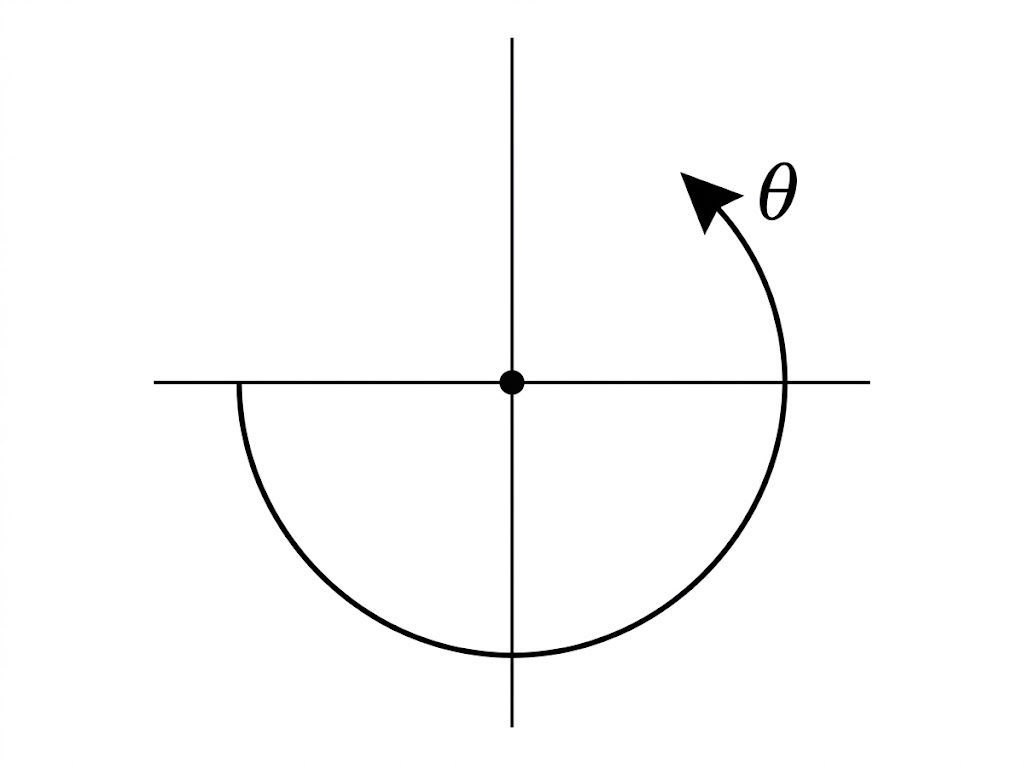
\includegraphics[scale=0.25]{pasted2}}
\par\end{center}

אז \L{%
\[
U_{1}=\left\{ \left(0,0\right)\right\} ,\quad U_{2}=\mathbb{R}^{2}
\]
}%
 הם כל התמ\textquotedblleft וים השמורים תחת \L{$T_{\theta}$}.

\subsubsection{הוכחה )לא היה בהרצאה(}

כיוון ראשון: בדוגמה {\beginL 1\endL} כבר הוכחנו ש-\L{$U_{1},U_{2}$}
הם תמ\textquotedblleft ו-ים שמורים תחת \L{$T_{\theta}$}.

כיוון שני: יהי \L{$W$} תמ\textquotedblleft ו שמור תחת \L{$T_{\theta}$}.

אם \L{$\dim(W)=0$} אז \L{$W=\left\{ v_{0}\right\} =U_{1}$}.

אם \L{$\dim(W)=1$} אז לכל בסיס של \L{$W$} יש בדיוק וקטור אחד שאינו
אפס ולכן קיים \L{$v_{0}\ne w\in W$} כך ש\L{%
\[
W=\text{Span}\left(w\right)=\left\{ cw:c\in\mathbb{R}\right\} 
\]
}%

היות ו-\L{$W$} תמ\textquotedblleft ו שמור,\L{%
\[
\forall v\in W,\ T_{\theta}(v)\in W
\]
}%
לכן

\L{%
\[
\forall v\in W\ \exists c\in\mathbb{R}\text{ s.t. }T_{\theta}(v)=cw
\]
}%

ובפרט, נסמן \L{$w=\left(a,b\right)$} ונקבל\L{%
\[
\exists c\in\mathbb{R}\text{ s.t. }cw=T_{\theta}(w)
\]
}%

מכאן\L{%
\[
\left(ca,cb\right)=aT_{\theta}(e_{1})+bT_{\theta}(e_{2})=\left(a\cos\theta-b\sin\theta,a\sin\theta+b\cos\theta\right)
\]
}%

כלומר

\L{%
\[
\begin{cases}
ca=a\cos\theta-b\sin\theta\\
cb=a\sin\theta+b\cos\theta
\end{cases}
\]
}%

מכאן\L{%
\[
\begin{cases}
cab=ab\cos\theta-b^{2}\sin\theta\\
cab=a^{2}\sin\theta+ab\cos\theta
\end{cases}
\]
}%

לכן\L{%
\[
a^{2}\sin\theta=-b^{2}\sin\theta\ \Rightarrow\ \left(a^{2}+b^{2}\right)\sin\theta=0\ \underset{\left(a,b\right)\ne\left(0,0\right)}{\Rightarrow}\ \sin\theta=0
\]
}%

בסתירה לכך ש-\L{$\theta\notin\left\{ k\pi:k\in\mathbb{Z}\right\} $}.

אם \L{$\dim(W)=2$} אז ניזכר שתמ\textquotedblleft ו של מ\textquotedblleft ו
נוצר סופית מאותו מימד שווה למ\textquotedblleft ו על כן \L{$W=U_{2}$}.

היות ומימד של תמ\textquotedblleft ו נ\textquotedblleft ס קטן או שווה
למימד של המ\textquotedblleft ו, אין עוד מקרים לבדוק וסיימנו.

\subsection{דוגמה{\normalsize{} }{\normalsize{\beginL 4}\endL}{\normalsize{} )טענה:
גרעין וטווח הם תמ\textquotedblleft ו שמורים תחת \L{$T$}(}}

יהי \L{$V$} מ\textquotedblleft ו מעל \L{$\mathbb{F}$} ותהא \L{$T\in\mathcal{L}(V)$}.

אז \L{$\text{Null}(T)$} ו-\L{$\text{Range}(T)$} הם תמיד תמ\textquotedblleft וים
שמורים תחת \L{$T$}.

\subsubsection{הוכחה )כן היה בהרצאה(}

לכל \L{$v\in\text{Null}(T)$} מתקיים \L{$T(V)=0_{V}$}, אבל \L{$0_{V}\in\text{Null}\left(T\right)$}
כי זה תמ\textquotedblleft ו, לכן זה תמ\textquotedblleft ו שמור תחת
\L{$T$}.

בנוסף, לכל \L{$v\in\text{Range}(T)$} מהגדרת הטווח, קיים \L{$v'\in V$}
כך ש- \L{$T(v')=v\in V$}.

אז גם \L{$T\left(v\right)=T\left(T\left(v'\right)\right)\in\text{Range}(T)$}
כנדרש.

\part{על אילו שאלות אנו מנסים לענות}

יהי \L{$T\in\mathcal{L}(V)$}.
\begin{enumerate}
\item[)I(] מהם תת-מרחבים השמורים תחת \L{$T$}? 
\item[)II(] כיצד ניתן לאפיין אותם? 
\item[)III(] כיצד תת-מרחבים השמורים תחת \L{$T$} מאפשרים לקבל הצגה מטריציאלית
הפשוטה ככל האפשר עבור \L{$T$}? 
\end{enumerate}
שאלה \L{$\left(\text{III}\right)$} היא המשמעותית ביותר. 

\textquotedblleft הפשוטה ככל האפשר\textquotedblright , הווה אומר,
כאשר כמה שיותר מספרים במטריצה שווים ל-{\beginL 0\endL}.

לכל אופרטור יש מטריצה מייצגת ביחס לבסיס מסוים - נחפש את הבסיסים שיאפשרו
את המטריצה המייצגת הפשוטה ביותר )שאפשר לראות מה היא עושה לכל וקטור
רק מלהסתכל( - זאת האידיאולוגיה בקורס.

כמובן, הכל תלוי בשדה ובתמ\textquotedblright ו. 

נחפש בסיסים נכונים 

\section{דוגמה וטענה - קריטריון מטריציוני לתמ\textquotedblright ו שמור}

\L{$V$} - מרחב מעל \L{$\mathbb{F}$}, \L{$\dim V=n\geq2$}, \L{$T\in\mathcal{L}(V)$}.

\L{$\mathcal{B}_{V}=(v_{1},\dots,v_{n})$} בסיס במרחב \L{$V$}. \L{%
\[
M(T,\mathcal{B}_{V},\mathcal{B}_{V})\overset{\text{def}}{=}(a_{i,j})_{i,j=1}^{n}
\]
}%
כאשר \L{%
\[
T(v_{j})=\sum_{i=1}^{n}a_{i,j}v_{i},\quad1\leq j\leq n
\]
}%

)זו המטריצה המייצגת \L{$\left[T\right]_{\mathcal{B}}^{\mathcal{B}}$}
מלינארית {\beginL 1\endL} - העמודה ה-\L{$j$} היא \L{$\left[T\left(v_{j}\right)\right]_{\mathcal{B}}$}.

הסימון \L{$M\left(T,\mathcal{B},\mathcal{B}\right)$} הוא הסימון של
אקסלר.(

נניח כי \L{%
\[
M(T,\mathcal{B}_{V},\mathcal{B}_{V})=\left(\begin{array}{ccc|ccc}
a_{1,1} & \cdots & a_{1,k} & a_{1,k+1} & \cdots & a_{1,n}\\
\vdots &  & \vdots & \vdots &  & \vdots\\
a_{k,1} & \cdots & a_{k,k} & a_{k,k+1} & \cdots & a_{k,n}\\
\hline 0_{\mathbb{F}} & \cdots & 0_{\mathbb{F}} & a_{k+1,k+1} & \cdots & a_{k+1,n}\\
\vdots &  & \vdots & \vdots &  & \vdots\\
0_{\mathbb{F}} & \cdots & 0_{\mathbb{F}} & a_{n,k+1} & \cdots & a_{n,n}
\end{array}\right)
\]
}%
)למשל \L{$a_{k+1,1}=0_{\mathbb{F}}$}(.

כלומר, \L{$a_{i,j}=0_{\mathbb{F}}$} לכל \L{$i>k$} ו-\L{$j\le k$}
עבור \L{$1\le k<n$} כלשהו.

אז התמ\textquotedblright ו \L{$U=\text{Span}(v_{1},\dots,v_{k})$}
הוא תמ\textquotedblright ו שמור תחת \L{$T$}.

\subsection{הוכחה}
\begin{enumerate}
\item ~ \L{%
\begin{align*}
T(v_{1}) & =a_{1,1}v_{1}+\dots+a_{k,1}v_{k}+\underset{=0_{\mathbb{F}}}{\underbrace{a_{k+1,1}}}v_{k+1}+\dots+\underset{=0_{\mathbb{F}}}{\underbrace{a_{n,1}}}v_{n}\\
 & \vdots\\
T(v_{k}) & =a_{1,k}v_{1}+\dots+a_{k,k}v_{k}+\underset{=0_{\mathbb{F}}}{\underbrace{a_{k+1,k}}}v_{k+1}+\dots+\underset{=0_{\mathbb{F}}}{\underbrace{a_{n,k}}}v_{n}
\end{align*}
}%
\item לכן \L{$T(v_{1}),\dots,T(v_{k})\in\text{Span}(v_{1},\dots,v_{k})$}
\item נניח כי \L{$u\in U$}. אזי \L{$u=d_{1}v_{1}+\dots+d_{k}v_{k}$} ומתקיים
\L{%
\[
T(u)=T(d_{1}v_{1}+\dots+d_{k}v_{k})=d_{1}T(v_{1})+\dots+d_{k}T(v_{k})
\]
}%
אבל \L{%
\[
T(v_{1})\in\text{Span}(v_{1},\dots,v_{k})
\]
}%
\L{%
\[
\vdots
\]
}%
\L{%
\[
T(v_{k})\in\text{Span}(v_{1},\dots,v_{k})
\]
}%
\L{%
\[
T(u)\in\underset{=U}{\underbrace{\text{Span}(v_{1},\dots,v_{k})}}\quad\Leftarrow
\]
}%
\hfill{}\L{$\blacksquare$}
\end{enumerate}
)לא היה בהרצאה( גם הכיוון ההפוך נכון: אם \L{$U$} תמ\textquotedblright ו
שמור תחת \L{$T$}, אז לכל \L{$j\le k$} מתקיים \L{$T(v_{j})\in\text{Span\ensuremath{\left(v_{1},\dots,v_{k}\right)}}$}
ומיחידות ההצגה לפי בסיס, לכל \L{$i>k$} מתקיים \L{$a_{i.j}=0_{\mathbb{F}}$}.

\subsection{הערה}

אם נניח כי בנוסף 

\L{%
\begin{align*}
 & a_{1,k+1}=\dots=a_{1,n}=0_{\mathbb{F}}\\
 & \vdots\\
 & a_{k,k+1}=\dots=a_{k,n}=0_{\mathbb{F}}
\end{align*}
}%

כלומר \L{%
\[
M(T,\mathcal{B}_{V},\mathcal{B}_{V})=\left(\begin{array}{c|c}
* & 0\\
\hline 0 & *
\end{array}\right)
\]
}%
אזי נקבל ש-\L{$U_{2}=\text{Span}(v_{k+1},\dots,v_{n})$} הוא תת-מרחב
שמור תחת \L{$T$}, וגם מתקיים \L{%
\[
V=U_{1}\oplus U_{2}
\]
}%

\section{משפט - סכום ישר של תמ\textquotedblright וים שמורים נותן מטריצה אלכסונית
בבלוקים}

יהי \L{$V$} מ\textquotedblright ו מעל \L{$\mathbb{F}$} עם \L{$\dim V=n$}
כך ש- \L{$n\geq2$}.

אם \L{$U_{1}$} ו-\L{$U_{2}$} שניהם תמ\textquotedblright וים שמורים
תחת \L{$T$} כך שמתקיים \L{$V=U_{1}\oplus U_{2}$} אז קיים בסיס \L{$\mathcal{B}_{V}$}
כך שמתקיים\L{%
\[
M(T,\mathcal{B}_{V},\mathcal{B}_{V})=\left(\begin{array}{ccc|ccc}
a_{1,1} & \cdots & a_{1,k} & 0_{\mathbb{F}} & \cdots & 0_{\mathbb{F}}\\
\vdots &  & \vdots & \vdots &  & \vdots\\
a_{k,1} & \cdots & a_{k,k} & 0_{\mathbb{F}} & \cdots & 0_{\mathbb{F}}\\
\hline 0_{\mathbb{F}} & \cdots & 0_{\mathbb{F}} & a_{k+1,k+1} & \cdots & a_{k+1,n}\\
\vdots &  & \vdots & \vdots &  & \vdots\\
0_{\mathbb{F}} & \cdots & 0_{\mathbb{F}} & a_{n,k+1} & \cdots & a_{n,n}
\end{array}\right)
\]
}%

\subsection{הוכחה}

נבחר בסיס \L{$\mathcal{B}_{U_{1}}=(v_{1},\dots,v_{k})$} ונבחר בסיס
\L{$\mathcal{B}_{U_{2}}=(v_{k+1},\dots,v_{n})$}.

מאחר ש-\L{$V=U_{1}\oplus U_{2}$}, מתקיים \L{$U_{1}\cap U_{2}=\{0_{V}\}$}
וגם \L{$\dim U_{1}+\dim U_{2}=\dim V$}, לכן \L{%
\[
\mathcal{B}_{V}=(v_{1},\dots,v_{k},v_{k+1},\dots,v_{n})
\]
}%

הוא בסיס של \L{$V$}. אבל בגלל שאלו תמ\textquotedblright וים שמורים
נקבל

\L{%
\begin{align*}
T(v_{1}) & =a_{1,1}v_{1}+\dots+a_{k,1}v_{k}+0_{\mathbb{F}}v_{k+1}+\dots+0_{\mathbb{F}}v_{n}\in U_{1}\\
 & \vdots\\
T(v_{k}) & =a_{1,k}v_{1}+\dots+a_{k,k}v_{k}+0_{\mathbb{F}}v_{k+1}+\dots+0_{\mathbb{F}}v_{n}\in U_{1}\\
T(v_{k+1}) & =0_{\mathbb{F}}v_{1}+\dots+0_{\mathbb{F}}v_{k}+a_{k+1,k+1}v_{k+1}+\dots+a_{n,k+1}v_{n}\in U_{2}\\
 & \vdots\\
T(v_{n}) & =0_{\mathbb{F}}v_{1}+\dots+0_{\mathbb{F}}v_{k}+a_{k+1,n}v_{k+1}+\dots+a_{n,n}v_{n}\in U_{2}
\end{align*}
}%

כנדרש.

\hfill{}\L{$\blacksquare$}

\part{ערך עצמי של אופרטור}

\section{הגדרה - ערך עצמי של אופרטור }

יהי \L{$V$} מ\textquotedblright ו מעל \L{$\mathbb{F}$}.

עבור אופרטור \L{$T\in\mathcal{L}(V)$}, אם קיים וקטור \L{$0_{V}\ne v\in V$}
כך שמתקיים \L{%
\[
T(v)=\lambda v
\]
}%
כאשר \L{$\lambda\in\mathbb{F}$}, נאמר כי \L{$\lambda$} הוא ערך עצמי
)\L{$\text{Eigenvalue}$}( של \L{$T$}.

\section{הגדרה - וקטור עצמי}

לכל \L{$v$} כזה נקרא וקטור עצמי של \L{$T$} השייך ל-\L{$\lambda$}. 

\section{תוספות מהכותב}

\L{$\left[\clubsuit\right]$} ערך עצמי מוגדר לפי אופרטור ו-וקטור עצמי
מוגדר לפי ערך עצמי.

\L{$\left[\spadesuit\right]$} ערך עצמי מגדיר תמ\textquotedblright ו
של \L{$V$} הנקרא מרחב עצמי )\L{$\text{Eigenspace}$}( \L{%
\[
E_{\lambda}(T)=\left\{ v\in V:T(v)=\lambda v\right\} 
\]
}%
עבור \L{$u,w\in E_{\lambda}(T)$}, \L{$c\in\mathbb{F}$} מתקיים\L{%
\[
T(u+cw)\underset{\text{T isa LT}}{=}T(u)+cT(w)\underset{\text{eigenspace property}}{=}\lambda u+c\lambda w=\lambda(u+cw)
\]
}%

כלומר המרחב סגור לחיבור וכפל בסקלר.

בנוסף,\L{%
\[
T(0)=\lambda\cdot0
\]
}%
לכן \L{$0\in E_{\lambda}(T)$}. )אסור להגדיר ערך עצמי בעזרת וקטור
האפס כי אז כל ערך יהיה ערך עצמי, אבל ברגע שכבר יש ערך עצמי זה טריוויאלי
שוקטור האפס שייך למרחב העצמי שהוא משרה(.
\end{document}
